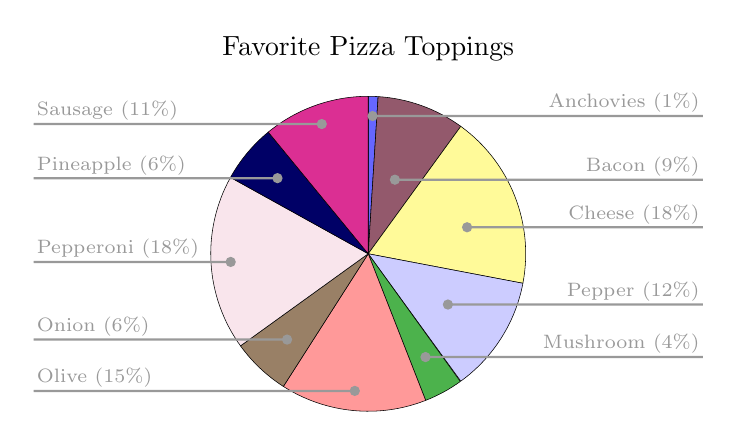
\begin{tikzpicture}
    
    % top of ring
    \filldraw[fill=blue!60!white,draw=black,very thin] (90:0) -- (90:2) arc (90:86.4:2) -- (86.4:0);
    \filldraw[purple!30!gray,draw=black,very thin] (86.4:0)--(86.4:2) arc (86.4:54:2)--(54:0);
    \filldraw[yellow!40!white,draw=black,very thin] (54:0) -- (54:2) arc (54:-10.8:2) -- (-10.8:0);
    \filldraw[blue!20!white,draw=black,very thin] (-10.8:0) -- (-10.8:2) arc (-10.8:-54:2) -- (-54.2:0);
    \filldraw[green!40!gray,draw=black,very thin] (-54.2:0) -- (-54.2:2) arc (-54.2:-68.6:2) -- (-68.6:0);
    \filldraw[red!40!white,draw=black,very thin] (-68.6:0) -- (-68.6:2) arc (-68.6:-122.6:2) -- (-122.6:0);
    \filldraw[orange!20!gray,draw=black,very thin] (-122.6:0) -- (-122.6:2) arc (-122.6:-144.2:2) -- (-144.2:0);
    \filldraw[purple!10!white,draw=black,very thin] (-144.2:0) -- (-144.2:2) arc (-144.2:-209:2) -- (-209:0);
    \filldraw[blue!40!black,draw=black,very thin] (-209:0) -- (-209:2) arc (-209:-230.6:2) -- (-230.6:0);
    \filldraw[magenta!80!gray,draw=black,very thin] (-230.6:0) -- (-230.6:2) arc (-230.6:-270:2) -- (-270:0);



    % top dividing lines between colors
    % \draw[very thin] (77:0cm) -- (77:1cm)
    %   (-5:0cm) -- (-5:1cm)
    %   (-112:0cm) -- (-112:1cm)
    %   (126:0cm) -- (126:1cm)
    %   (0,0) circle (1cm);
    %  (90:0.5cm)  arc (90 :135:0.5cm);

    % establish coordinates for reference below
    \coordinate (left border) at (4.25,0); 
    \coordinate (right border) at (-4.25,0); 
    \coordinate (l1) at (88.2:1.75);
    \coordinate (l2) at (70.2:1); 
    \coordinate (l3) at (15:1.3);
    \coordinate (l4) at (-32.5:1.2);
    \coordinate (l5) at (-61:1.5);
    \coordinate (l6) at (-95.6:1.75);
    \coordinate (l7) at (-133.4:1.5);
    \coordinate (l8) at (-176.6:1.75);
    \coordinate (l9) at (-219.8:1.5);
    \coordinate (l10) at (-250.3:1.75);

    % attach labels
    \begin{scope}[lab/.style={gray!80!white,thick,draw,font={\scriptsize}},outer sep=-0.75mm]
      % \fill[lab] (l1) circle(0.05) -- (l1-|left border) node[anchor=south east] {Anchovies} node[anchor=north east] {1\%};
      % \fill[lab] (l2) circle(0.05) -- (l2-|left border) node[anchor=south east] {Bacon} node[anchor=north east] {9\%}; 
      % \fill[lab] (l3) circle(0.05) -- (l3-|left border) node[anchor=south east] {Cheese} node[anchor=north east] {18\%};
      % \fill[lab] (l4) circle(0.05) -- (l4-|left border) node[anchor=south east] {Pepper} node[anchor=north east] {12\%}; 
      % \fill[lab] (l5) circle(0.05) -- (l5-|left border) node[anchor=south east] {Mushroom} node[anchor=north east] {4\%};
      % \fill[lab] (l6) circle(0.05) -- (l6-|right border) node[anchor=south west] {Olive} node[anchor=north west] {15\%}; 
      % \fill[lab] (l7) circle(0.05) -- (l7-|right border) node[anchor=south west] {Onion} node[anchor=north west] {6\%}; 
      \fill[lab] (l1) circle(0.05) -- (l1-|left border) node[anchor=south east] {Anchovies (1\%)};
      \fill[lab] (l2) circle(0.05) -- (l2-|left border) node[anchor=south east] {Bacon (9\%)}; 
      \fill[lab] (l3) circle(0.05) -- (l3-|left border) node[anchor=south east] {Cheese (18\%)};
      \fill[lab] (l4) circle(0.05) -- (l4-|left border) node[anchor=south east] {Pepper (12\%)}; 
      \fill[lab] (l5) circle(0.05) -- (l5-|left border) node[anchor=south east] {Mushroom (4\%)};
      \fill[lab] (l6) circle(0.05) -- (l6-|right border) node[anchor=south west] {Olive (15\%)}; 
      \fill[lab] (l7) circle(0.05) -- (l7-|right border) node[anchor=south west] {Onion (6\%)};
      \fill[lab] (l8) circle(0.05) -- (l8-|right border) node[anchor=south west] {Pepperoni (18\%)};
      \fill[lab] (l9) circle(0.05) -- (l9-|right border) node[anchor=south west] {Pineapple (6\%)};
      \fill[lab] (l10) circle(0.05) -- (l10-|right border) node[anchor=south west] {Sausage (11\%)};
    \end{scope}
    
    % Title
    \node at (0,2.6) {Favorite Pizza Toppings};
\end{tikzpicture}    